\documentclass{article}

\usepackage{graphicx}
\usepackage{tikz}
\usepackage{tikzsymbols}
\usetikzlibrary{calc,patterns,shapes.geometric}
\pagestyle{empty}
\usepackage[margin=0pt]{geometry}
\geometry{papersize={14in,12in}}

\def\centerarc[#1](#2)(#3:#4:#5){\draw[#1] ($(#2)+({#5*cos(#3)},{#5*sin(#3)})$) arc (#3:#4:#5);}

\begin{document}
	\begin{figure}
		\centering
		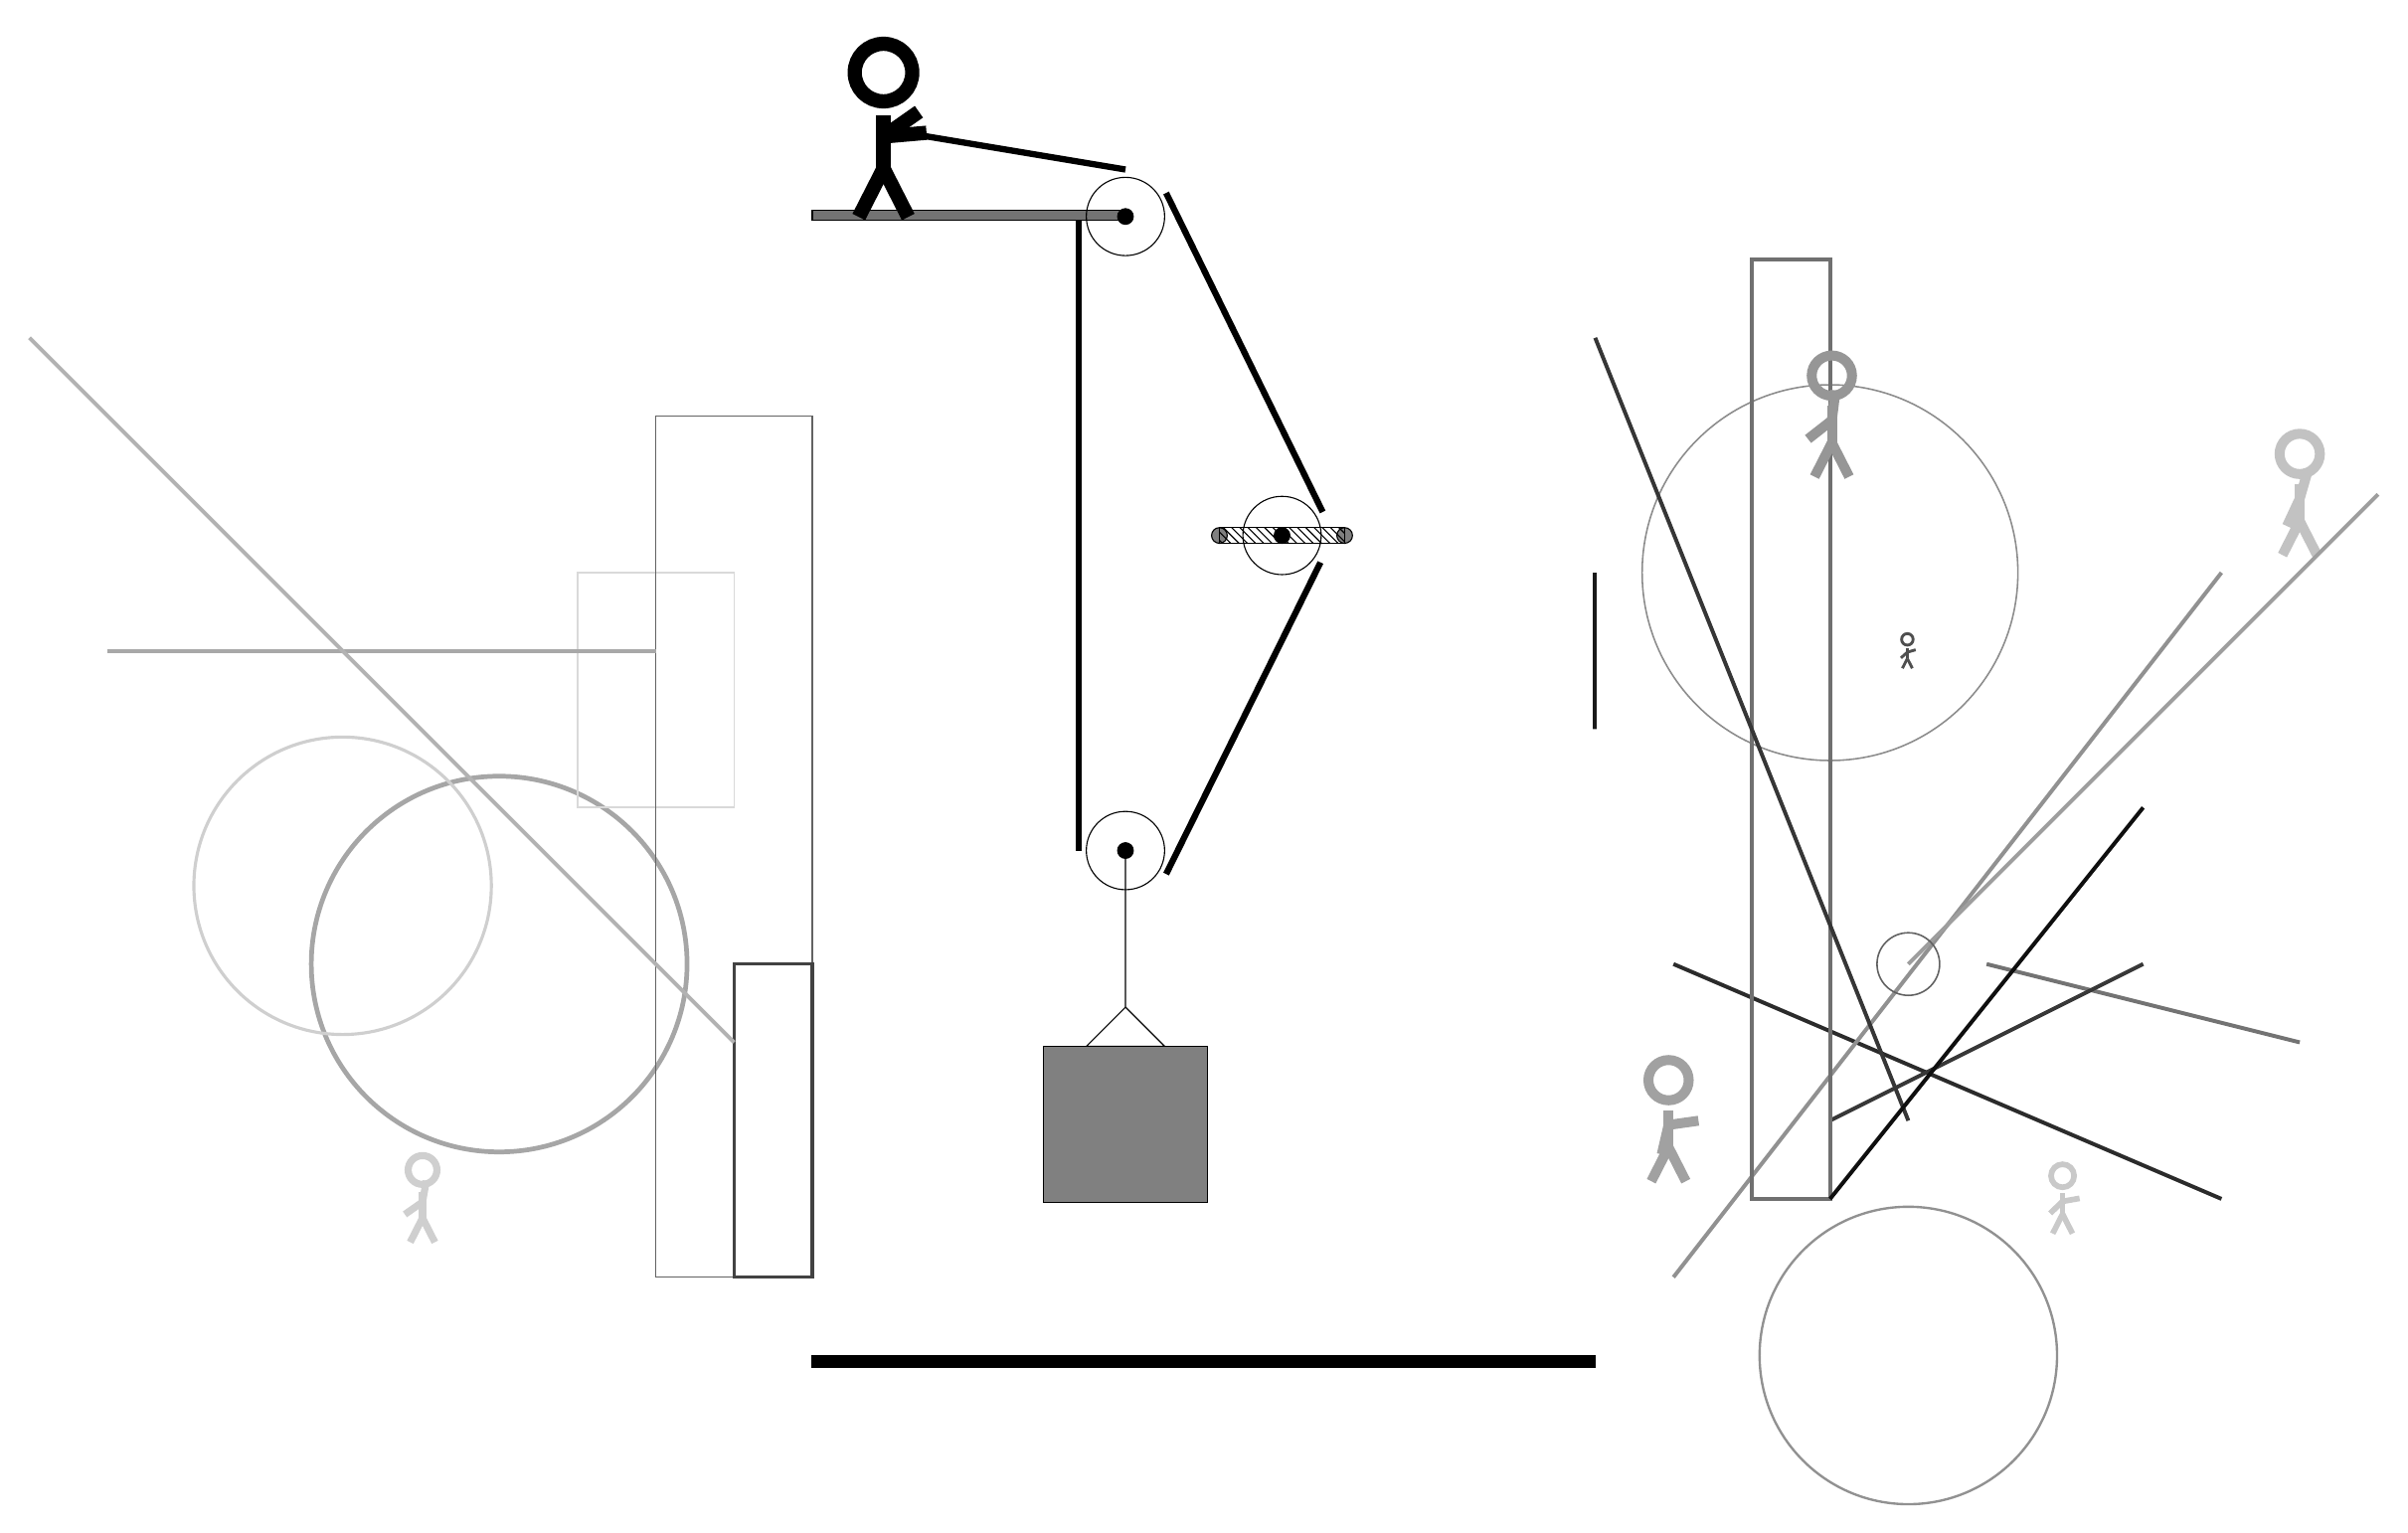
\begin{tikzpicture}
			%%%%% START %%%%%
			
			\draw[fill=black!55] (-2, 11.5) rectangle (2, 11.625);
			
			\draw (2, 3.45) circle (0.5);
			\draw[fill=black] (2, 3.45) circle (0.1);
			
			\draw (2, 11.55) circle (0.5);
			\draw[fill=black] (2, 11.55) circle (0.1);
			
			\draw[fill=white](4, 7.475) circle (0.5);
			\draw[fill=black] (4, 7.475) circle (0.1);
			\draw[fill=black!50] (3.2, 7.475) circle (0.1);
			\draw[fill=black!50] (4.8, 7.475) circle (0.1);
			\draw[pattern=north west lines, pattern color=black] (3.2, 7.575) rectangle (4.8, 7.375);
			
			\draw (2, 3.45) -- (2, 1.45) -- (1.5, 0.95) -- (2.5, 0.95) -- (2, 1.45);
			\draw[fill=black!50] (0.95, 0.95) rectangle (3.05, -1.05);
			
			\draw[line width=0.8mm] (1.4, 11.5) -- (1.4, 3.45);
			\centerarc[line width=0.8mm](2, 3.45)(180:330:0.6);
			\draw[line width=0.8mm](2.5196, 3.15) -- (4.4915, 7.1308);
			\centerarc[line width=0.8mm](4, 7.475)(390:325:0.6);
			\draw[line width=0.8mm](4.5196, 7.775) -- (2.5196, 11.85);
			\centerarc[line width=0.8mm](2, 11.55)(30:90:0.6);
			\draw[line width=0.8mm](2, 12.15) -- (-1, 12.65);
			
			\node at (-1, 12.65) {\Strichmaxerl[10][-175][35]};
			
			\node[line width=0.5mm, color=black!21] at (14, -1) {\Strichmaxerl[4][44][10]};
			
			\draw[line width=0.5mm, color=black!83](9, 2) -- (16, -1);
			\draw[line width=0.5mm, color=black!43](9, -2) -- (16, 7);
			\draw[line width=0.5mm, color=black!55](13, 2) -- (17, 1);
			\draw [line width=0.2mm, color=black!45](11, 7) circle (2.4);
			\draw[line width=0.5mm, color=black!78](11, 0) -- (15, 2);
			\draw [line width=0.6mm, color=black!35](-6, 2) circle (2.4);
			\draw[line width=0.2mm, color=black!15] (-3, 7) rectangle (-5, 4);
			\node[line width=0.7mm, color=black!69] at (12, 6) {\Strichmaxerl[2][42][16]};
			
			\draw[line width=0.2mm, color=black!61] (-4, 9) rectangle (-2, -2);
			\draw[line width=0.5mm, color=black!56] (10, 11) rectangle (11, -1);
			\draw[line width=0.5mm, color=black!34](-4, 6) -- (-11, 6);
			\node[line width=0.7mm, color=black!24] at (17, 8) {\Strichmaxerl[7][65][74]};
			
			\draw [line width=0.4mm, color=black!19](-8, 3) circle (1.9);
			\draw[line width=0.5mm, color=black!79](8, 10) -- (12, 0);
			\node[line width=0.2mm, color=black!19] at (-7, -1) {\Strichmaxerl[5][35][80]};
			
			\draw[line width=0.5mm, color=black!94](11, -1) -- (15, 4);
			\draw[line width=0.5mm, color=black!38](12, 2) -- (18, 8);
			\draw [line width=0.6mm, color=black!12](-7, 6) circle (0.0);
			\draw [line width=0.2mm, color=black!62](12, 2) circle (0.4);
			\node[line width=0.4mm, color=black!41] at (11, 9) {\Strichmaxerl[7][38][83]};
			
			\node[line width=0.3mm, color=black!37] at (9, 0) {\Strichmaxerl[7][77][8]};
			\draw[line width=0.4mm, color=black!74] (-3, 2) rectangle (-2, -2);
			\draw[line width=0.5mm, color=black!30](-3, 1) -- (-12, 10);
			\draw [line width=0.3mm, color=black!43](12, -3) circle (1.9);
			\draw[line width=0.5mm, color=black!90] (8, 5) rectangle (8, 7);
			
			\draw[fill=black] (-2, -3) rectangle (8, -3.15);
			
			%%%%% END %%%%%
		\end{tikzpicture}
	\end{figure}	
\end{document}